\documentclass[12pt]{extarticle}
\usepackage[T1]{fontenc}
\usepackage{tgheros}
\renewcommand{\familydefault}{\sfdefault}
\usepackage[letterpaper,left=0.75in,right=0.75in,top=0.8in,bottom=0.8in,
  headheight=16pt,headsep=16pt,footskip=28pt]{geometry}
\usepackage{tikz}
\definecolor{slotred}{RGB}{248,182,182}
\definecolor{slotblue}{RGB}{112,152,228}
\usepackage{array}
\usepackage{fancyhdr}
\pagestyle{fancy}
\fancyhf{}
\fancyhead[L]{\normalsize Week NN / Towers from either end / Grades 4--5}
\fancyfoot[L]{\small Bellingham Math Circle / Week NN / NN-45-v1}
\fancyfoot[R]{\small \thepage}
\renewcommand{\headrulewidth}{0pt}
\setlength{\parindent}{0pt}
\setlength{\parskip}{5pt}
\newcounter{prob}
\newcommand{\problem}{\par\bigskip\stepcounter{prob}\noindent\textbf{Problem \theprob:} }
\newcommand{\ruledlines}[2]{\par\noindent\begin{tikzpicture}
  \foreach \k in {1,...,#1}{\draw[black!35] (0,-\k*#2) -- (\linewidth-1pt,-\k*#2);}
  \end{tikzpicture}\par}
\begin{document}

Build the towers on a strip of slots. Two players take turns. On your turn,
take one whole tower from either end of the row. When the row is empty, the
player with more cubes wins. The same number of cubes is a tie. A row is
written as its tower heights from slot 1, so this row is 3, 1, 4, 2:
\par\smallskip
\centerline{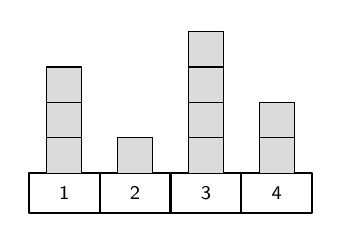
\begin{tikzpicture}[x=1mm,y=1mm,line join=round]
\path (0,0) rectangle (36,23.5);
\draw[thick, fill=white] (0,0) rectangle (9,5);
\node[font=\scriptsize] at (4.5,2.5) {1};
\draw[fill=black!14] (2.25,5.0) rectangle (6.75,9.5);
\draw[fill=black!14] (2.25,9.5) rectangle (6.75,14.0);
\draw[fill=black!14] (2.25,14.0) rectangle (6.75,18.5);
\draw[thick, fill=white] (9,0) rectangle (18,5);
\node[font=\scriptsize] at (13.5,2.5) {2};
\draw[fill=black!14] (11.25,5.0) rectangle (15.75,9.5);
\draw[thick, fill=white] (18,0) rectangle (27,5);
\node[font=\scriptsize] at (22.5,2.5) {3};
\draw[fill=black!14] (20.25,5.0) rectangle (24.75,9.5);
\draw[fill=black!14] (20.25,9.5) rectangle (24.75,14.0);
\draw[fill=black!14] (20.25,14.0) rectangle (24.75,18.5);
\draw[fill=black!14] (20.25,18.5) rectangle (24.75,23.0);
\draw[thick, fill=white] (27,0) rectangle (36,5);
\node[font=\scriptsize] at (31.5,2.5) {4};
\draw[fill=black!14] (29.25,5.0) rectangle (33.75,9.5);
\draw[fill=black!14] (29.25,9.5) rectangle (33.75,14.0);
\end{tikzpicture}\hspace{6mm}\raisebox{6mm}{\tikz[x=1mm,y=1mm]\draw[-latex, black!60, thick] (0,0) -- (9,0);}\hspace{6mm}\raisebox{3mm}{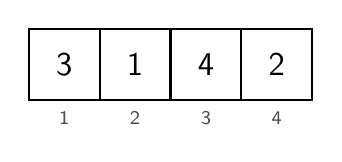
\begin{tikzpicture}[x=1mm,y=1mm]
\draw[thick, fill=white] (0,0) rectangle (9,9);
\node[font=\large] at (4.5,4.5) {3};
\node[font=\scriptsize, black!70] at (4.5,-2.3) {1};
\draw[thick, fill=white] (9,0) rectangle (18,9);
\node[font=\large] at (13.5,4.5) {1};
\node[font=\scriptsize, black!70] at (13.5,-2.3) {2};
\draw[thick, fill=white] (18,0) rectangle (27,9);
\node[font=\large] at (22.5,4.5) {4};
\node[font=\scriptsize, black!70] at (22.5,-2.3) {3};
\draw[thick, fill=white] (27,0) rectangle (36,9);
\node[font=\large] at (31.5,4.5) {2};
\node[font=\scriptsize, black!70] at (31.5,-2.3) {4};
\end{tikzpicture}}}
\par\smallskip
Playing as well as you can means collecting as many cubes as you can be sure
of. Who wins a row, and by how many cubes, means the result when both players
play as well as they can.
\problem For each row, find who wins and by how many cubes. Write each player's total.\par\vspace{2mm}\centerline{{\renewcommand{\arraystretch}{1.8}\begin{tabular}{l@{\hspace{8mm}}l@{\hspace{2mm}}p{13mm}@{\hspace{5mm}}l@{\hspace{2mm}}p{13mm}}
2, 1, 5, 3 & first player & \hrulefill & second player & \hrulefill\\
1, 4, 6, 2 & first player & \hrulefill & second player & \hrulefill\\
2, 4, 3, 1 & first player & \hrulefill & second player & \hrulefill\\
6, 2, 1, 5 & first player & \hrulefill & second player & \hrulefill\\
\end{tabular}}}\par\problem Who wins each row of three? Write each player's total. Find a rule that tells you who wins from the three heights, and explain why it works.\par\vspace{2mm}\centerline{{\renewcommand{\arraystretch}{1.8}\begin{tabular}{l@{\hspace{8mm}}l@{\hspace{2mm}}p{13mm}@{\hspace{5mm}}l@{\hspace{2mm}}p{13mm}}
1, 5, 1 & first player & \hrulefill & second player & \hrulefill\\
5, 1, 5 & first player & \hrulefill & second player & \hrulefill\\
2, 6, 3 & first player & \hrulefill & second player & \hrulefill\\
3, 4, 2 & first player & \hrulefill & second player & \hrulefill\\
2, 5, 3 & first player & \hrulefill & second player & \hrulefill\\
6, 1, 2 & first player & \hrulefill & second player & \hrulefill\\
\end{tabular}}}\par\ruledlines{4}{8mm}\newpage\problem Is there a row of four towers, each 1 to 6 cubes high, on which the first player loses?\par\vspace{2mm}\vspace{4mm}\noindent \begin{minipage}[b]{0.48\linewidth}\centering 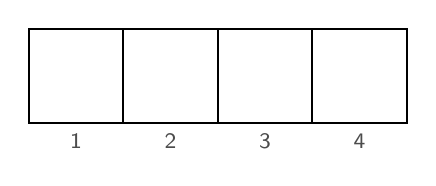
\begin{tikzpicture}[x=1mm,y=1mm]
\draw[thick, fill=white] (0,0) rectangle (12,12);
\node[font=\footnotesize, black!70] at (6.0,-2.3) {1};
\draw[thick, fill=white] (12,0) rectangle (24,12);
\node[font=\footnotesize, black!70] at (18.0,-2.3) {2};
\draw[thick, fill=white] (24,0) rectangle (36,12);
\node[font=\footnotesize, black!70] at (30.0,-2.3) {3};
\draw[thick, fill=white] (36,0) rectangle (48,12);
\node[font=\footnotesize, black!70] at (42.0,-2.3) {4};
\end{tikzpicture}\end{minipage}\hfill\begin{minipage}[b]{0.48\linewidth}\centering 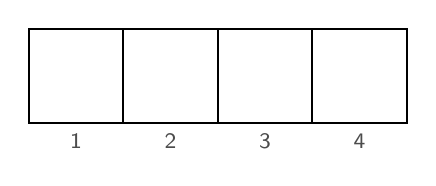
\begin{tikzpicture}[x=1mm,y=1mm]
\draw[thick, fill=white] (0,0) rectangle (12,12);
\node[font=\footnotesize, black!70] at (6.0,-2.3) {1};
\draw[thick, fill=white] (12,0) rectangle (24,12);
\node[font=\footnotesize, black!70] at (18.0,-2.3) {2};
\draw[thick, fill=white] (24,0) rectangle (36,12);
\node[font=\footnotesize, black!70] at (30.0,-2.3) {3};
\draw[thick, fill=white] (36,0) rectangle (48,12);
\node[font=\footnotesize, black!70] at (42.0,-2.3) {4};
\end{tikzpicture}\end{minipage}\par\vspace{9mm}
\noindent \begin{minipage}[b]{0.48\linewidth}\centering 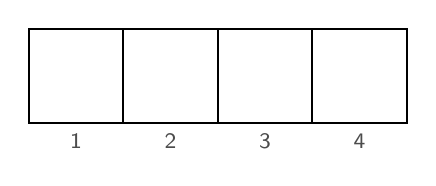
\begin{tikzpicture}[x=1mm,y=1mm]
\draw[thick, fill=white] (0,0) rectangle (12,12);
\node[font=\footnotesize, black!70] at (6.0,-2.3) {1};
\draw[thick, fill=white] (12,0) rectangle (24,12);
\node[font=\footnotesize, black!70] at (18.0,-2.3) {2};
\draw[thick, fill=white] (24,0) rectangle (36,12);
\node[font=\footnotesize, black!70] at (30.0,-2.3) {3};
\draw[thick, fill=white] (36,0) rectangle (48,12);
\node[font=\footnotesize, black!70] at (42.0,-2.3) {4};
\end{tikzpicture}\end{minipage}\hfill\begin{minipage}[b]{0.48\linewidth}\centering 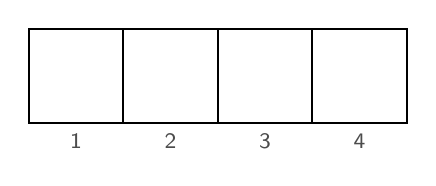
\begin{tikzpicture}[x=1mm,y=1mm]
\draw[thick, fill=white] (0,0) rectangle (12,12);
\node[font=\footnotesize, black!70] at (6.0,-2.3) {1};
\draw[thick, fill=white] (12,0) rectangle (24,12);
\node[font=\footnotesize, black!70] at (18.0,-2.3) {2};
\draw[thick, fill=white] (24,0) rectangle (36,12);
\node[font=\footnotesize, black!70] at (30.0,-2.3) {3};
\draw[thick, fill=white] (36,0) rectangle (48,12);
\node[font=\footnotesize, black!70] at (42.0,-2.3) {4};
\end{tikzpicture}\end{minipage}\par\vspace{9mm}
\noindent \begin{minipage}[b]{0.48\linewidth}\centering 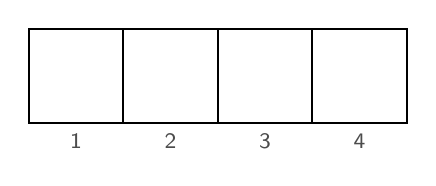
\begin{tikzpicture}[x=1mm,y=1mm]
\draw[thick, fill=white] (0,0) rectangle (12,12);
\node[font=\footnotesize, black!70] at (6.0,-2.3) {1};
\draw[thick, fill=white] (12,0) rectangle (24,12);
\node[font=\footnotesize, black!70] at (18.0,-2.3) {2};
\draw[thick, fill=white] (24,0) rectangle (36,12);
\node[font=\footnotesize, black!70] at (30.0,-2.3) {3};
\draw[thick, fill=white] (36,0) rectangle (48,12);
\node[font=\footnotesize, black!70] at (42.0,-2.3) {4};
\end{tikzpicture}\end{minipage}\hfill\begin{minipage}[b]{0.48\linewidth}\centering 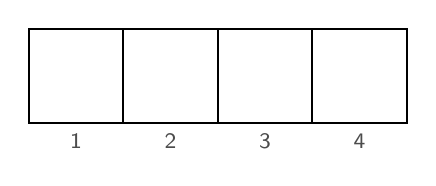
\begin{tikzpicture}[x=1mm,y=1mm]
\draw[thick, fill=white] (0,0) rectangle (12,12);
\node[font=\footnotesize, black!70] at (6.0,-2.3) {1};
\draw[thick, fill=white] (12,0) rectangle (24,12);
\node[font=\footnotesize, black!70] at (18.0,-2.3) {2};
\draw[thick, fill=white] (24,0) rectangle (36,12);
\node[font=\footnotesize, black!70] at (30.0,-2.3) {3};
\draw[thick, fill=white] (36,0) rectangle (48,12);
\node[font=\footnotesize, black!70] at (42.0,-2.3) {4};
\end{tikzpicture}\end{minipage}\par\vspace{9mm}
\noindent \begin{minipage}[b]{0.48\linewidth}\centering 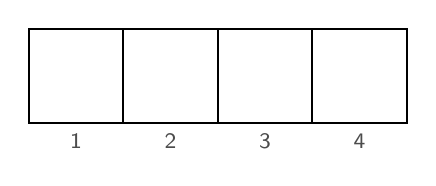
\begin{tikzpicture}[x=1mm,y=1mm]
\draw[thick, fill=white] (0,0) rectangle (12,12);
\node[font=\footnotesize, black!70] at (6.0,-2.3) {1};
\draw[thick, fill=white] (12,0) rectangle (24,12);
\node[font=\footnotesize, black!70] at (18.0,-2.3) {2};
\draw[thick, fill=white] (24,0) rectangle (36,12);
\node[font=\footnotesize, black!70] at (30.0,-2.3) {3};
\draw[thick, fill=white] (36,0) rectangle (48,12);
\node[font=\footnotesize, black!70] at (42.0,-2.3) {4};
\end{tikzpicture}\end{minipage}\hfill\begin{minipage}[b]{0.48\linewidth}\centering 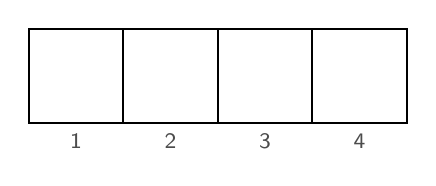
\begin{tikzpicture}[x=1mm,y=1mm]
\draw[thick, fill=white] (0,0) rectangle (12,12);
\node[font=\footnotesize, black!70] at (6.0,-2.3) {1};
\draw[thick, fill=white] (12,0) rectangle (24,12);
\node[font=\footnotesize, black!70] at (18.0,-2.3) {2};
\draw[thick, fill=white] (24,0) rectangle (36,12);
\node[font=\footnotesize, black!70] at (30.0,-2.3) {3};
\draw[thick, fill=white] (36,0) rectangle (48,12);
\node[font=\footnotesize, black!70] at (42.0,-2.3) {4};
\end{tikzpicture}\end{minipage}\par\vspace{9mm}\ruledlines{6}{9mm}\newpage\problem The grown-up goes first on the colored strips and never loses. Play these rows against the grown-up as a team, and work out the grown-up's plan.\par\vspace{4mm}\noindent\hfill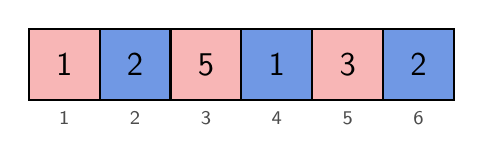
\begin{tikzpicture}[x=1mm,y=1mm]
\draw[thick, fill=slotred] (0,0) rectangle (9,9);
\node[font=\large] at (4.5,4.5) {1};
\node[font=\scriptsize, black!70] at (4.5,-2.3) {1};
\draw[thick, fill=slotblue] (9,0) rectangle (18,9);
\node[font=\large] at (13.5,4.5) {2};
\node[font=\scriptsize, black!70] at (13.5,-2.3) {2};
\draw[thick, fill=slotred] (18,0) rectangle (27,9);
\node[font=\large] at (22.5,4.5) {5};
\node[font=\scriptsize, black!70] at (22.5,-2.3) {3};
\draw[thick, fill=slotblue] (27,0) rectangle (36,9);
\node[font=\large] at (31.5,4.5) {1};
\node[font=\scriptsize, black!70] at (31.5,-2.3) {4};
\draw[thick, fill=slotred] (36,0) rectangle (45,9);
\node[font=\large] at (40.5,4.5) {3};
\node[font=\scriptsize, black!70] at (40.5,-2.3) {5};
\draw[thick, fill=slotblue] (45,0) rectangle (54,9);
\node[font=\large] at (49.5,4.5) {2};
\node[font=\scriptsize, black!70] at (49.5,-2.3) {6};
\end{tikzpicture}\hfill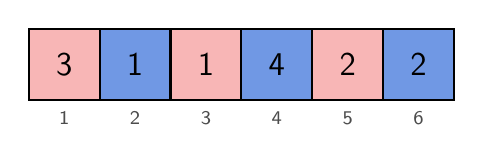
\begin{tikzpicture}[x=1mm,y=1mm]
\draw[thick, fill=slotred] (0,0) rectangle (9,9);
\node[font=\large] at (4.5,4.5) {3};
\node[font=\scriptsize, black!70] at (4.5,-2.3) {1};
\draw[thick, fill=slotblue] (9,0) rectangle (18,9);
\node[font=\large] at (13.5,4.5) {1};
\node[font=\scriptsize, black!70] at (13.5,-2.3) {2};
\draw[thick, fill=slotred] (18,0) rectangle (27,9);
\node[font=\large] at (22.5,4.5) {1};
\node[font=\scriptsize, black!70] at (22.5,-2.3) {3};
\draw[thick, fill=slotblue] (27,0) rectangle (36,9);
\node[font=\large] at (31.5,4.5) {4};
\node[font=\scriptsize, black!70] at (31.5,-2.3) {4};
\draw[thick, fill=slotred] (36,0) rectangle (45,9);
\node[font=\large] at (40.5,4.5) {2};
\node[font=\scriptsize, black!70] at (40.5,-2.3) {5};
\draw[thick, fill=slotblue] (45,0) rectangle (54,9);
\node[font=\large] at (49.5,4.5) {2};
\node[font=\scriptsize, black!70] at (49.5,-2.3) {6};
\end{tikzpicture}\hfill\null\par\vspace{5mm}\centerline{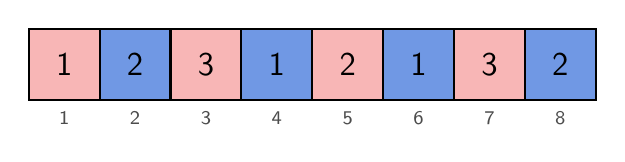
\begin{tikzpicture}[x=1mm,y=1mm]
\draw[thick, fill=slotred] (0,0) rectangle (9,9);
\node[font=\large] at (4.5,4.5) {1};
\node[font=\scriptsize, black!70] at (4.5,-2.3) {1};
\draw[thick, fill=slotblue] (9,0) rectangle (18,9);
\node[font=\large] at (13.5,4.5) {2};
\node[font=\scriptsize, black!70] at (13.5,-2.3) {2};
\draw[thick, fill=slotred] (18,0) rectangle (27,9);
\node[font=\large] at (22.5,4.5) {3};
\node[font=\scriptsize, black!70] at (22.5,-2.3) {3};
\draw[thick, fill=slotblue] (27,0) rectangle (36,9);
\node[font=\large] at (31.5,4.5) {1};
\node[font=\scriptsize, black!70] at (31.5,-2.3) {4};
\draw[thick, fill=slotred] (36,0) rectangle (45,9);
\node[font=\large] at (40.5,4.5) {2};
\node[font=\scriptsize, black!70] at (40.5,-2.3) {5};
\draw[thick, fill=slotblue] (45,0) rectangle (54,9);
\node[font=\large] at (49.5,4.5) {1};
\node[font=\scriptsize, black!70] at (49.5,-2.3) {6};
\draw[thick, fill=slotred] (54,0) rectangle (63,9);
\node[font=\large] at (58.5,4.5) {3};
\node[font=\scriptsize, black!70] at (58.5,-2.3) {7};
\draw[thick, fill=slotblue] (63,0) rectangle (72,9);
\node[font=\large] at (67.5,4.5) {2};
\node[font=\scriptsize, black!70] at (67.5,-2.3) {8};
\end{tikzpicture}}\par\ruledlines{4}{8mm}\problem Explain why the grown-up's plan never loses on a row with an even number of towers, whatever the other player does.\par\vspace{2mm}\ruledlines{8}{8.5mm}\newpage\problem In each of these colored rows, the red slots and the blue slots hold the same number of cubes. Which rows can the first player win, and by how many cubes?\par\vspace{4mm}\noindent \begin{minipage}[b]{0.32\linewidth}\centering 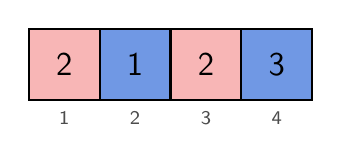
\begin{tikzpicture}[x=1mm,y=1mm]
\draw[thick, fill=slotred] (0,0) rectangle (9,9);
\node[font=\large] at (4.5,4.5) {2};
\node[font=\scriptsize, black!70] at (4.5,-2.3) {1};
\draw[thick, fill=slotblue] (9,0) rectangle (18,9);
\node[font=\large] at (13.5,4.5) {1};
\node[font=\scriptsize, black!70] at (13.5,-2.3) {2};
\draw[thick, fill=slotred] (18,0) rectangle (27,9);
\node[font=\large] at (22.5,4.5) {2};
\node[font=\scriptsize, black!70] at (22.5,-2.3) {3};
\draw[thick, fill=slotblue] (27,0) rectangle (36,9);
\node[font=\large] at (31.5,4.5) {3};
\node[font=\scriptsize, black!70] at (31.5,-2.3) {4};
\end{tikzpicture}\\[3mm]{\small first \rule{11mm}{0.4pt}\quad second \rule{11mm}{0.4pt}}\end{minipage}\hfill\begin{minipage}[b]{0.32\linewidth}\centering 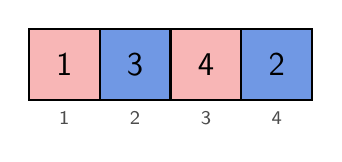
\begin{tikzpicture}[x=1mm,y=1mm]
\draw[thick, fill=slotred] (0,0) rectangle (9,9);
\node[font=\large] at (4.5,4.5) {1};
\node[font=\scriptsize, black!70] at (4.5,-2.3) {1};
\draw[thick, fill=slotblue] (9,0) rectangle (18,9);
\node[font=\large] at (13.5,4.5) {3};
\node[font=\scriptsize, black!70] at (13.5,-2.3) {2};
\draw[thick, fill=slotred] (18,0) rectangle (27,9);
\node[font=\large] at (22.5,4.5) {4};
\node[font=\scriptsize, black!70] at (22.5,-2.3) {3};
\draw[thick, fill=slotblue] (27,0) rectangle (36,9);
\node[font=\large] at (31.5,4.5) {2};
\node[font=\scriptsize, black!70] at (31.5,-2.3) {4};
\end{tikzpicture}\\[3mm]{\small first \rule{11mm}{0.4pt}\quad second \rule{11mm}{0.4pt}}\end{minipage}\hfill\begin{minipage}[b]{0.32\linewidth}\centering 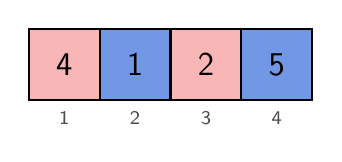
\begin{tikzpicture}[x=1mm,y=1mm]
\draw[thick, fill=slotred] (0,0) rectangle (9,9);
\node[font=\large] at (4.5,4.5) {4};
\node[font=\scriptsize, black!70] at (4.5,-2.3) {1};
\draw[thick, fill=slotblue] (9,0) rectangle (18,9);
\node[font=\large] at (13.5,4.5) {1};
\node[font=\scriptsize, black!70] at (13.5,-2.3) {2};
\draw[thick, fill=slotred] (18,0) rectangle (27,9);
\node[font=\large] at (22.5,4.5) {2};
\node[font=\scriptsize, black!70] at (22.5,-2.3) {3};
\draw[thick, fill=slotblue] (27,0) rectangle (36,9);
\node[font=\large] at (31.5,4.5) {5};
\node[font=\scriptsize, black!70] at (31.5,-2.3) {4};
\end{tikzpicture}\\[3mm]{\small first \rule{11mm}{0.4pt}\quad second \rule{11mm}{0.4pt}}\end{minipage}\par\vspace{7mm}
\noindent \begin{minipage}[b]{0.32\linewidth}\centering 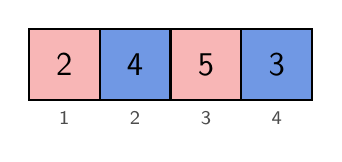
\begin{tikzpicture}[x=1mm,y=1mm]
\draw[thick, fill=slotred] (0,0) rectangle (9,9);
\node[font=\large] at (4.5,4.5) {2};
\node[font=\scriptsize, black!70] at (4.5,-2.3) {1};
\draw[thick, fill=slotblue] (9,0) rectangle (18,9);
\node[font=\large] at (13.5,4.5) {4};
\node[font=\scriptsize, black!70] at (13.5,-2.3) {2};
\draw[thick, fill=slotred] (18,0) rectangle (27,9);
\node[font=\large] at (22.5,4.5) {5};
\node[font=\scriptsize, black!70] at (22.5,-2.3) {3};
\draw[thick, fill=slotblue] (27,0) rectangle (36,9);
\node[font=\large] at (31.5,4.5) {3};
\node[font=\scriptsize, black!70] at (31.5,-2.3) {4};
\end{tikzpicture}\\[3mm]{\small first \rule{11mm}{0.4pt}\quad second \rule{11mm}{0.4pt}}\end{minipage}\hfill\begin{minipage}[b]{0.32\linewidth}\centering 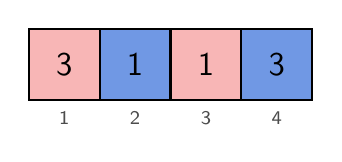
\begin{tikzpicture}[x=1mm,y=1mm]
\draw[thick, fill=slotred] (0,0) rectangle (9,9);
\node[font=\large] at (4.5,4.5) {3};
\node[font=\scriptsize, black!70] at (4.5,-2.3) {1};
\draw[thick, fill=slotblue] (9,0) rectangle (18,9);
\node[font=\large] at (13.5,4.5) {1};
\node[font=\scriptsize, black!70] at (13.5,-2.3) {2};
\draw[thick, fill=slotred] (18,0) rectangle (27,9);
\node[font=\large] at (22.5,4.5) {1};
\node[font=\scriptsize, black!70] at (22.5,-2.3) {3};
\draw[thick, fill=slotblue] (27,0) rectangle (36,9);
\node[font=\large] at (31.5,4.5) {3};
\node[font=\scriptsize, black!70] at (31.5,-2.3) {4};
\end{tikzpicture}\\[3mm]{\small first \rule{11mm}{0.4pt}\quad second \rule{11mm}{0.4pt}}\end{minipage}\hfill\begin{minipage}[b]{0.32\linewidth}\centering 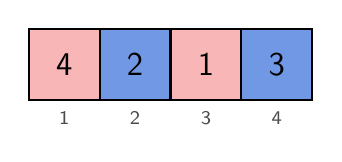
\begin{tikzpicture}[x=1mm,y=1mm]
\draw[thick, fill=slotred] (0,0) rectangle (9,9);
\node[font=\large] at (4.5,4.5) {4};
\node[font=\scriptsize, black!70] at (4.5,-2.3) {1};
\draw[thick, fill=slotblue] (9,0) rectangle (18,9);
\node[font=\large] at (13.5,4.5) {2};
\node[font=\scriptsize, black!70] at (13.5,-2.3) {2};
\draw[thick, fill=slotred] (18,0) rectangle (27,9);
\node[font=\large] at (22.5,4.5) {1};
\node[font=\scriptsize, black!70] at (22.5,-2.3) {3};
\draw[thick, fill=slotblue] (27,0) rectangle (36,9);
\node[font=\large] at (31.5,4.5) {3};
\node[font=\scriptsize, black!70] at (31.5,-2.3) {4};
\end{tikzpicture}\\[3mm]{\small first \rule{11mm}{0.4pt}\quad second \rule{11mm}{0.4pt}}\end{minipage}\par\vspace{7mm}\problem In each of these colored rows of five, the blue slots hold more cubes than the red slots. Who wins each row? Explain why.\par\vspace{4mm}\noindent \begin{minipage}[b]{0.48\linewidth}\centering 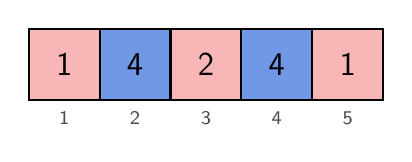
\begin{tikzpicture}[x=1mm,y=1mm]
\draw[thick, fill=slotred] (0,0) rectangle (9,9);
\node[font=\large] at (4.5,4.5) {1};
\node[font=\scriptsize, black!70] at (4.5,-2.3) {1};
\draw[thick, fill=slotblue] (9,0) rectangle (18,9);
\node[font=\large] at (13.5,4.5) {4};
\node[font=\scriptsize, black!70] at (13.5,-2.3) {2};
\draw[thick, fill=slotred] (18,0) rectangle (27,9);
\node[font=\large] at (22.5,4.5) {2};
\node[font=\scriptsize, black!70] at (22.5,-2.3) {3};
\draw[thick, fill=slotblue] (27,0) rectangle (36,9);
\node[font=\large] at (31.5,4.5) {4};
\node[font=\scriptsize, black!70] at (31.5,-2.3) {4};
\draw[thick, fill=slotred] (36,0) rectangle (45,9);
\node[font=\large] at (40.5,4.5) {1};
\node[font=\scriptsize, black!70] at (40.5,-2.3) {5};
\end{tikzpicture}\\[3mm]{\small first \rule{11mm}{0.4pt}\quad second \rule{11mm}{0.4pt}}\end{minipage}\hfill\begin{minipage}[b]{0.48\linewidth}\centering 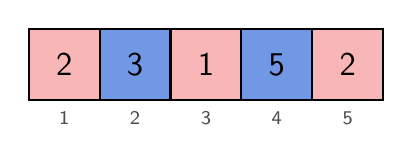
\begin{tikzpicture}[x=1mm,y=1mm]
\draw[thick, fill=slotred] (0,0) rectangle (9,9);
\node[font=\large] at (4.5,4.5) {2};
\node[font=\scriptsize, black!70] at (4.5,-2.3) {1};
\draw[thick, fill=slotblue] (9,0) rectangle (18,9);
\node[font=\large] at (13.5,4.5) {3};
\node[font=\scriptsize, black!70] at (13.5,-2.3) {2};
\draw[thick, fill=slotred] (18,0) rectangle (27,9);
\node[font=\large] at (22.5,4.5) {1};
\node[font=\scriptsize, black!70] at (22.5,-2.3) {3};
\draw[thick, fill=slotblue] (27,0) rectangle (36,9);
\node[font=\large] at (31.5,4.5) {5};
\node[font=\scriptsize, black!70] at (31.5,-2.3) {4};
\draw[thick, fill=slotred] (36,0) rectangle (45,9);
\node[font=\large] at (40.5,4.5) {2};
\node[font=\scriptsize, black!70] at (40.5,-2.3) {5};
\end{tikzpicture}\\[3mm]{\small first \rule{11mm}{0.4pt}\quad second \rule{11mm}{0.4pt}}\end{minipage}\par\vspace{6mm}
\noindent \begin{minipage}[b]{0.48\linewidth}\centering 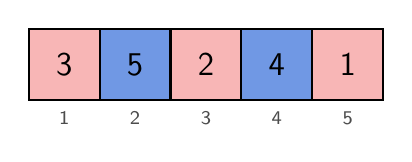
\begin{tikzpicture}[x=1mm,y=1mm]
\draw[thick, fill=slotred] (0,0) rectangle (9,9);
\node[font=\large] at (4.5,4.5) {3};
\node[font=\scriptsize, black!70] at (4.5,-2.3) {1};
\draw[thick, fill=slotblue] (9,0) rectangle (18,9);
\node[font=\large] at (13.5,4.5) {5};
\node[font=\scriptsize, black!70] at (13.5,-2.3) {2};
\draw[thick, fill=slotred] (18,0) rectangle (27,9);
\node[font=\large] at (22.5,4.5) {2};
\node[font=\scriptsize, black!70] at (22.5,-2.3) {3};
\draw[thick, fill=slotblue] (27,0) rectangle (36,9);
\node[font=\large] at (31.5,4.5) {4};
\node[font=\scriptsize, black!70] at (31.5,-2.3) {4};
\draw[thick, fill=slotred] (36,0) rectangle (45,9);
\node[font=\large] at (40.5,4.5) {1};
\node[font=\scriptsize, black!70] at (40.5,-2.3) {5};
\end{tikzpicture}\\[3mm]{\small first \rule{11mm}{0.4pt}\quad second \rule{11mm}{0.4pt}}\end{minipage}\hfill\begin{minipage}[b]{0.48\linewidth}\centering 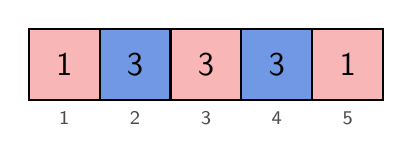
\begin{tikzpicture}[x=1mm,y=1mm]
\draw[thick, fill=slotred] (0,0) rectangle (9,9);
\node[font=\large] at (4.5,4.5) {1};
\node[font=\scriptsize, black!70] at (4.5,-2.3) {1};
\draw[thick, fill=slotblue] (9,0) rectangle (18,9);
\node[font=\large] at (13.5,4.5) {3};
\node[font=\scriptsize, black!70] at (13.5,-2.3) {2};
\draw[thick, fill=slotred] (18,0) rectangle (27,9);
\node[font=\large] at (22.5,4.5) {3};
\node[font=\scriptsize, black!70] at (22.5,-2.3) {3};
\draw[thick, fill=slotblue] (27,0) rectangle (36,9);
\node[font=\large] at (31.5,4.5) {3};
\node[font=\scriptsize, black!70] at (31.5,-2.3) {4};
\draw[thick, fill=slotred] (36,0) rectangle (45,9);
\node[font=\large] at (40.5,4.5) {1};
\node[font=\scriptsize, black!70] at (40.5,-2.3) {5};
\end{tikzpicture}\\[3mm]{\small first \rule{11mm}{0.4pt}\quad second \rule{11mm}{0.4pt}}\end{minipage}\par\vspace{6mm}\ruledlines{5}{8mm}\newpage\problem In each of these colored rows of five, the red slots hold more cubes than the blue slots. Who wins each row?\par\vspace{4mm}\noindent \begin{minipage}[b]{0.48\linewidth}\centering 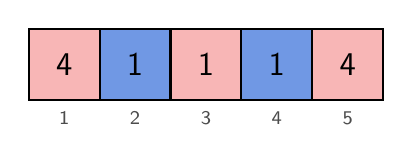
\begin{tikzpicture}[x=1mm,y=1mm]
\draw[thick, fill=slotred] (0,0) rectangle (9,9);
\node[font=\large] at (4.5,4.5) {4};
\node[font=\scriptsize, black!70] at (4.5,-2.3) {1};
\draw[thick, fill=slotblue] (9,0) rectangle (18,9);
\node[font=\large] at (13.5,4.5) {1};
\node[font=\scriptsize, black!70] at (13.5,-2.3) {2};
\draw[thick, fill=slotred] (18,0) rectangle (27,9);
\node[font=\large] at (22.5,4.5) {1};
\node[font=\scriptsize, black!70] at (22.5,-2.3) {3};
\draw[thick, fill=slotblue] (27,0) rectangle (36,9);
\node[font=\large] at (31.5,4.5) {1};
\node[font=\scriptsize, black!70] at (31.5,-2.3) {4};
\draw[thick, fill=slotred] (36,0) rectangle (45,9);
\node[font=\large] at (40.5,4.5) {4};
\node[font=\scriptsize, black!70] at (40.5,-2.3) {5};
\end{tikzpicture}\\[3mm]{\small first \rule{11mm}{0.4pt}\quad second \rule{11mm}{0.4pt}}\end{minipage}\hfill\begin{minipage}[b]{0.48\linewidth}\centering 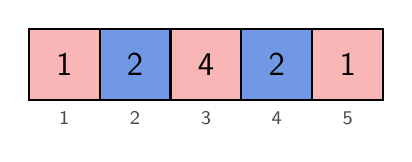
\begin{tikzpicture}[x=1mm,y=1mm]
\draw[thick, fill=slotred] (0,0) rectangle (9,9);
\node[font=\large] at (4.5,4.5) {1};
\node[font=\scriptsize, black!70] at (4.5,-2.3) {1};
\draw[thick, fill=slotblue] (9,0) rectangle (18,9);
\node[font=\large] at (13.5,4.5) {2};
\node[font=\scriptsize, black!70] at (13.5,-2.3) {2};
\draw[thick, fill=slotred] (18,0) rectangle (27,9);
\node[font=\large] at (22.5,4.5) {4};
\node[font=\scriptsize, black!70] at (22.5,-2.3) {3};
\draw[thick, fill=slotblue] (27,0) rectangle (36,9);
\node[font=\large] at (31.5,4.5) {2};
\node[font=\scriptsize, black!70] at (31.5,-2.3) {4};
\draw[thick, fill=slotred] (36,0) rectangle (45,9);
\node[font=\large] at (40.5,4.5) {1};
\node[font=\scriptsize, black!70] at (40.5,-2.3) {5};
\end{tikzpicture}\\[3mm]{\small first \rule{11mm}{0.4pt}\quad second \rule{11mm}{0.4pt}}\end{minipage}\par\vspace{6mm}
\noindent \begin{minipage}[b]{0.48\linewidth}\centering 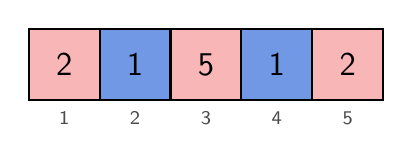
\begin{tikzpicture}[x=1mm,y=1mm]
\draw[thick, fill=slotred] (0,0) rectangle (9,9);
\node[font=\large] at (4.5,4.5) {2};
\node[font=\scriptsize, black!70] at (4.5,-2.3) {1};
\draw[thick, fill=slotblue] (9,0) rectangle (18,9);
\node[font=\large] at (13.5,4.5) {1};
\node[font=\scriptsize, black!70] at (13.5,-2.3) {2};
\draw[thick, fill=slotred] (18,0) rectangle (27,9);
\node[font=\large] at (22.5,4.5) {5};
\node[font=\scriptsize, black!70] at (22.5,-2.3) {3};
\draw[thick, fill=slotblue] (27,0) rectangle (36,9);
\node[font=\large] at (31.5,4.5) {1};
\node[font=\scriptsize, black!70] at (31.5,-2.3) {4};
\draw[thick, fill=slotred] (36,0) rectangle (45,9);
\node[font=\large] at (40.5,4.5) {2};
\node[font=\scriptsize, black!70] at (40.5,-2.3) {5};
\end{tikzpicture}\\[3mm]{\small first \rule{11mm}{0.4pt}\quad second \rule{11mm}{0.4pt}}\end{minipage}\hfill\begin{minipage}[b]{0.48\linewidth}\centering 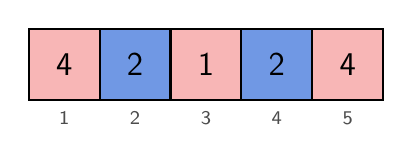
\begin{tikzpicture}[x=1mm,y=1mm]
\draw[thick, fill=slotred] (0,0) rectangle (9,9);
\node[font=\large] at (4.5,4.5) {4};
\node[font=\scriptsize, black!70] at (4.5,-2.3) {1};
\draw[thick, fill=slotblue] (9,0) rectangle (18,9);
\node[font=\large] at (13.5,4.5) {2};
\node[font=\scriptsize, black!70] at (13.5,-2.3) {2};
\draw[thick, fill=slotred] (18,0) rectangle (27,9);
\node[font=\large] at (22.5,4.5) {1};
\node[font=\scriptsize, black!70] at (22.5,-2.3) {3};
\draw[thick, fill=slotblue] (27,0) rectangle (36,9);
\node[font=\large] at (31.5,4.5) {2};
\node[font=\scriptsize, black!70] at (31.5,-2.3) {4};
\draw[thick, fill=slotred] (36,0) rectangle (45,9);
\node[font=\large] at (40.5,4.5) {4};
\node[font=\scriptsize, black!70] at (40.5,-2.3) {5};
\end{tikzpicture}\\[3mm]{\small first \rule{11mm}{0.4pt}\quad second \rule{11mm}{0.4pt}}\end{minipage}\par\vspace{6mm}
\noindent \begin{minipage}[b]{0.48\linewidth}\centering 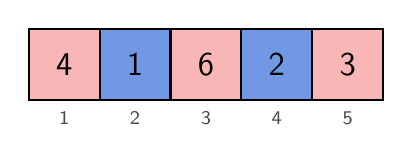
\begin{tikzpicture}[x=1mm,y=1mm]
\draw[thick, fill=slotred] (0,0) rectangle (9,9);
\node[font=\large] at (4.5,4.5) {4};
\node[font=\scriptsize, black!70] at (4.5,-2.3) {1};
\draw[thick, fill=slotblue] (9,0) rectangle (18,9);
\node[font=\large] at (13.5,4.5) {1};
\node[font=\scriptsize, black!70] at (13.5,-2.3) {2};
\draw[thick, fill=slotred] (18,0) rectangle (27,9);
\node[font=\large] at (22.5,4.5) {6};
\node[font=\scriptsize, black!70] at (22.5,-2.3) {3};
\draw[thick, fill=slotblue] (27,0) rectangle (36,9);
\node[font=\large] at (31.5,4.5) {2};
\node[font=\scriptsize, black!70] at (31.5,-2.3) {4};
\draw[thick, fill=slotred] (36,0) rectangle (45,9);
\node[font=\large] at (40.5,4.5) {3};
\node[font=\scriptsize, black!70] at (40.5,-2.3) {5};
\end{tikzpicture}\\[3mm]{\small first \rule{11mm}{0.4pt}\quad second \rule{11mm}{0.4pt}}\end{minipage}\hfill\null\par\vspace{6mm}\problem Can the first player win a row of five on which the red slots and the blue slots hold the same number of cubes? Explain.\par\vspace{2mm}\ruledlines{6}{8mm}\newpage\problem For each row, ring the first player's best first move, and find who wins and by how many cubes.\par\vspace{4mm}\noindent \begin{minipage}[b]{0.32\linewidth}\centering 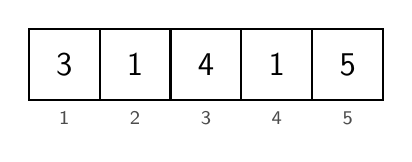
\begin{tikzpicture}[x=1mm,y=1mm]
\draw[thick, fill=white] (0,0) rectangle (9,9);
\node[font=\large] at (4.5,4.5) {3};
\node[font=\scriptsize, black!70] at (4.5,-2.3) {1};
\draw[thick, fill=white] (9,0) rectangle (18,9);
\node[font=\large] at (13.5,4.5) {1};
\node[font=\scriptsize, black!70] at (13.5,-2.3) {2};
\draw[thick, fill=white] (18,0) rectangle (27,9);
\node[font=\large] at (22.5,4.5) {4};
\node[font=\scriptsize, black!70] at (22.5,-2.3) {3};
\draw[thick, fill=white] (27,0) rectangle (36,9);
\node[font=\large] at (31.5,4.5) {1};
\node[font=\scriptsize, black!70] at (31.5,-2.3) {4};
\draw[thick, fill=white] (36,0) rectangle (45,9);
\node[font=\large] at (40.5,4.5) {5};
\node[font=\scriptsize, black!70] at (40.5,-2.3) {5};
\end{tikzpicture}\\[3mm]{\small first \rule{11mm}{0.4pt}\quad second \rule{11mm}{0.4pt}}\end{minipage}\hfill\begin{minipage}[b]{0.32\linewidth}\centering 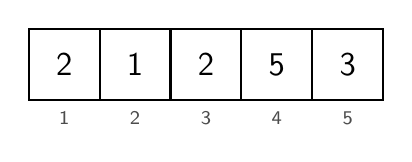
\begin{tikzpicture}[x=1mm,y=1mm]
\draw[thick, fill=white] (0,0) rectangle (9,9);
\node[font=\large] at (4.5,4.5) {2};
\node[font=\scriptsize, black!70] at (4.5,-2.3) {1};
\draw[thick, fill=white] (9,0) rectangle (18,9);
\node[font=\large] at (13.5,4.5) {1};
\node[font=\scriptsize, black!70] at (13.5,-2.3) {2};
\draw[thick, fill=white] (18,0) rectangle (27,9);
\node[font=\large] at (22.5,4.5) {2};
\node[font=\scriptsize, black!70] at (22.5,-2.3) {3};
\draw[thick, fill=white] (27,0) rectangle (36,9);
\node[font=\large] at (31.5,4.5) {5};
\node[font=\scriptsize, black!70] at (31.5,-2.3) {4};
\draw[thick, fill=white] (36,0) rectangle (45,9);
\node[font=\large] at (40.5,4.5) {3};
\node[font=\scriptsize, black!70] at (40.5,-2.3) {5};
\end{tikzpicture}\\[3mm]{\small first \rule{11mm}{0.4pt}\quad second \rule{11mm}{0.4pt}}\end{minipage}\hfill\begin{minipage}[b]{0.32\linewidth}\centering 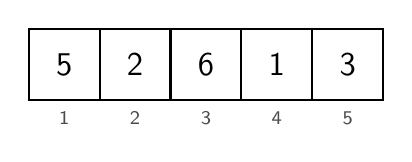
\begin{tikzpicture}[x=1mm,y=1mm]
\draw[thick, fill=white] (0,0) rectangle (9,9);
\node[font=\large] at (4.5,4.5) {5};
\node[font=\scriptsize, black!70] at (4.5,-2.3) {1};
\draw[thick, fill=white] (9,0) rectangle (18,9);
\node[font=\large] at (13.5,4.5) {2};
\node[font=\scriptsize, black!70] at (13.5,-2.3) {2};
\draw[thick, fill=white] (18,0) rectangle (27,9);
\node[font=\large] at (22.5,4.5) {6};
\node[font=\scriptsize, black!70] at (22.5,-2.3) {3};
\draw[thick, fill=white] (27,0) rectangle (36,9);
\node[font=\large] at (31.5,4.5) {1};
\node[font=\scriptsize, black!70] at (31.5,-2.3) {4};
\draw[thick, fill=white] (36,0) rectangle (45,9);
\node[font=\large] at (40.5,4.5) {3};
\node[font=\scriptsize, black!70] at (40.5,-2.3) {5};
\end{tikzpicture}\\[3mm]{\small first \rule{11mm}{0.4pt}\quad second \rule{11mm}{0.4pt}}\end{minipage}\par\vspace{4mm}\problem In each box, write the most cubes the player whose turn it is can be sure of collecting from that row, in a game on 2, 3, 6, 2, 1, 4.\par\vspace{5mm}\centerline{\begin{tikzpicture}[x=1mm,y=1mm]
\draw[black!75] (0.0,0.0) rectangle (27.5,15.0);
\node[font=\footnotesize, anchor=north] at (13.75,14.4) {2};
\draw[black!75] (29.1,0.0) rectangle (56.6,15.0);
\node[font=\footnotesize, anchor=north] at (42.85,14.4) {3};
\draw[black!75] (58.2,0.0) rectangle (85.7,15.0);
\node[font=\footnotesize, anchor=north] at (71.95,14.4) {6};
\draw[black!75] (87.30000000000001,0.0) rectangle (114.80000000000001,15.0);
\node[font=\footnotesize, anchor=north] at (101.05000000000001,14.4) {2};
\draw[black!75] (116.4,0.0) rectangle (143.9,15.0);
\node[font=\footnotesize, anchor=north] at (130.15,14.4) {1};
\draw[black!75] (145.5,0.0) rectangle (173.0,15.0);
\node[font=\footnotesize, anchor=north] at (159.25,14.4) {4};
\draw[black!75] (14.549999999999997,17.4) rectangle (42.05,32.4);
\node[font=\footnotesize, anchor=north] at (28.299999999999997,31.799999999999997) {2,\,3};
\draw[black!75] (43.65,17.4) rectangle (71.15,32.4);
\node[font=\footnotesize, anchor=north] at (57.4,31.799999999999997) {3,\,6};
\draw[black!75] (72.75,17.4) rectangle (100.25,32.4);
\node[font=\footnotesize, anchor=north] at (86.5,31.799999999999997) {6,\,2};
\draw[black!75] (101.85000000000001,17.4) rectangle (129.35000000000002,32.4);
\node[font=\footnotesize, anchor=north] at (115.60000000000001,31.799999999999997) {2,\,1};
\draw[black!75] (130.95,17.4) rectangle (158.45,32.4);
\node[font=\footnotesize, anchor=north] at (144.7,31.799999999999997) {1,\,4};
\draw[black!75] (29.1,34.8) rectangle (56.6,49.8);
\node[font=\footnotesize, anchor=north] at (42.85,49.199999999999996) {2,\,3,\,6};
\draw[black!75] (58.2,34.8) rectangle (85.7,49.8);
\node[font=\footnotesize, anchor=north] at (71.95,49.199999999999996) {3,\,6,\,2};
\draw[black!75] (87.30000000000001,34.8) rectangle (114.80000000000001,49.8);
\node[font=\footnotesize, anchor=north] at (101.05000000000001,49.199999999999996) {6,\,2,\,1};
\draw[black!75] (116.4,34.8) rectangle (143.9,49.8);
\node[font=\footnotesize, anchor=north] at (130.15,49.199999999999996) {2,\,1,\,4};
\draw[black!75] (43.65,52.199999999999996) rectangle (71.15,67.19999999999999);
\node[font=\footnotesize, anchor=north] at (57.4,66.6) {2,\,3,\,6,\,2};
\draw[black!75] (72.75,52.199999999999996) rectangle (100.25,67.19999999999999);
\node[font=\footnotesize, anchor=north] at (86.5,66.6) {3,\,6,\,2,\,1};
\draw[black!75] (101.85,52.199999999999996) rectangle (129.35,67.19999999999999);
\node[font=\footnotesize, anchor=north] at (115.6,66.6) {6,\,2,\,1,\,4};
\draw[black!75] (58.2,69.6) rectangle (85.7,84.6);
\node[font=\footnotesize, anchor=north] at (71.95,84.0) {2,\,3,\,6,\,2,\,1};
\draw[black!75] (87.30000000000001,69.6) rectangle (114.80000000000001,84.6);
\node[font=\footnotesize, anchor=north] at (101.05000000000001,84.0) {3,\,6,\,2,\,1,\,4};
\draw[black!75] (72.75,87.0) rectangle (100.25,102.0);
\node[font=\footnotesize, anchor=north] at (86.5,101.4) {2,\,3,\,6,\,2,\,1,\,4};
\end{tikzpicture}}\par
\end{document}
